%\documentclass[twocolumn, trackchanges]{aastex6}
\documentclass[preprint2]{aastex61}


\bibliographystyle{aasjournal}
\usepackage{graphicx}
\usepackage[suffix=]{epstopdf}
\usepackage{natbib}
\usepackage{amsmath}
\usepackage{url}
\usepackage{xspace}



%    Make Scientific Notation
\providecommand{\e}[1]{\ensuremath{\times 10^{#1}}}

% make the word Kepler italicized, deal w/ floating space afterwards
\newcommand{\Kepler}{\textsl{Kepler}\xspace}

\begin{document}

%%%%%%%%%%%%%%%%%%%%%%
\title{Constraining Starspot Latitudes with Transiting Exoplanets}

\shorttitle{Starspot Latitudes}
\shortauthors{Davenport et al.}


\author{James. R. A. Davenport}
\affiliation{Department of Astronomy, University of Washington, Seattle, WA 98195, USA}
\affiliation{NSF Astronomy and Astrophysics Postdoctoral Fellow}

\author{Brett M. Morris}
\affiliation{Department of Astronomy, University of Washington, Seattle, WA 98195, USA}

\author{Leslie Hebb}
\affiliation{Department of Physics, Hobart and William Smith Colleges, Geneva, NY, 14456}

\author{Michelle Gomez}
\affiliation{Department of Physics, Hobart and William Smith Colleges, Geneva, NY, 14456}

\author{Eric Agol}
\affiliation{Department of Astronomy, University of Washington, Seattle, WA 98195, USA}

\author{Suzanne L. Hawley}
\affiliation{Department of Astronomy, University of Washington, Seattle, WA 98195, USA}



%%%%%%%%%%%%%%%%%%%%%%%%%%%%%%
\begin{abstract}
Active latitude bands, as well as the ``Solar Butterfly Diagram'', are foundational properties that drive models of the solar dynamo. However, while considerable progress has been made on modeling stellar dynamos, no comparable constraint for the latitude distribution of active regions has been available. Here we present an ensemble approach to studying the latitude distribution of starspots using \Kepler transiting exoplanets. By exploiting the differences in impact parameter ($b$), the planets occult a range of latitude bands. We find X, using Y stars, and note Z. The future is bright.
\end{abstract}

\keywords{stars: activity}


%%%%%%%%%%%%%%%%%%%%%%%%%%%%%%
\section{Introduction}
\label{sec:intro}

The latitude where starspots form is a key component of stellar dynamo theory, but is a parameter that is nearly unconstrained with observations. We must therefore rely largely on the Sun for guidance. Starspots trace the surface magnetic field, and are therefore valuable for understanding the geometry and strength of the star's internal magnetic field \citep{berdyugina2005}.
For the Sun, spots predominantly form within two roughly symmetric bands of latitude centered about the equator. Throughout the 11-year solar activity cycle, the mean latitudes of these bands decreases towards the equator, from $\sim$$25^\circ$ to $\sim$$10^\circ$ (CITE). This sunspot latitude variation over time is known as the ``Butterfly Diagram'', first reported by \citet{maunder1904}.
``Active latitudes'', as on the Sun, occur as a result of stellar rotation and differential rotation, which governs the activity cycle length in the $\alpha\Omega$ mean-field dynamo model \citep{brandenburg2005}. The rate of stellar mass and angular momentum loss is also dependent on the surface magnetic field morphology \citep{garraffo2015}, and improvements in stellar spin-down models will require advances in surface field maps \citep{garraffo2016}.
Determining the latitudes of starspots is therefore vital for calibrating mean field dynamo theory from the Sun to other stars.


Despite a lack of information about starspot latitudes, much has been done to search for other observable constraints of a Solar-like dynamo.
Considerable effort has been made to search for overall magnetic activity cycles for stars, primarily in measuring chromospheric Ca II H\&K emission over decades \citep[e.g.]{wilson1978,baliunas1995}. These surveys require long baselines, but have yielded many possible activity cycles. While starspot modulation rotation curves have been measured for tens of thousands of stars using space-based photometric monitoring \citep{mcquillan2014}, differential rotation from via starspot modulations remains largely unconstrained \citep{aigrain2015}, with a few exceptions for rapidly rotating stars \citep[e.g.][]{davenport2015b}. 


Despite its importance, starspot latitudes have only been constrained for a handful of systems -- a natural result of stellar surfaces being unresolved due to their great distance. 
Coarse maps of the stellar magnetic field can be generated via Doppler Imaging techniques for rapidly rotating stars \citep{semel1989,donati_brown1997}, but typically cannot resolve small enough size scales to study individual spots comparable to those observed on the Sun.
For a small number of nearby active stars, the surface can be imaged directly via interferometry. \cite{roettenbacher2016} made use of this method to map the starspots on the old active star, $\zeta$ And, finding no sign of a solar-like spot distribution. Techniques for constraining starspot latitudes for larger samples of stars, particularly for older or slower rotating stars, are desperately needed.


Here we introduce a statistical approach to mapping the distribution of starspots as a function of stellar latitude. Transiting exoplanets have been previously used to probe the starspot activity along single latitude bands for individual stars. By exploiting the varying geometry for many transiting systems, specifically the impact parameter, we can create an ensemble picture of the latitudes where starspots are most prevalent. While the detailed geometry of each transiting planet+star system requires careful consideration when mapping back to stellar latitude, the method can be applied to a great number of transit hosts. This approach can be extended beyond single-band transit photometry, which will help measure detailed active region properties, and with extended monitoring campaigns of transits we may be able to simultaneously model the stellar activity cycles.



% idea discussed initially by: \cite{gomez2015}


%%%%%%%%%%%%%%%%%%%%%%
\section{Starspots from Transit Tomography}
\label{sec:transit}

Transiting exoplanets provide a unique means to detect small-scale surfaces features on stars. As the planet passes in front of the star, changing levels of flux on the stellar surface due to hot or cool regions affect the transit depth. In this ``transit tomography'', the planet provides a one-dimensional map of the surface brightness. When the planet passes over cool starspots, the transit depth is briefly shallower, resulting in ``bumps'' in the transit light curve \citep{silva2003}. The amplitude of these features are determined by the planet size relative to the star (which governs the overall transit depth), the starspot size relative to the planet, and the temperature contrast of the spot to the average photosphere. For bright, nearby stars with transiting Neptune or Jupiter sized planets, these bumps can reach $\sim$1/4 the transit depth, and the structure of individual spot groups can be studied. 

Missions like \Kepler now routinely observe transits with the photometric precision required to detect these bumps \citep{borucki2010}, and indeed many \Kepler systems have had their spot properties measured from this technique \citep[e.g.][]{sanchis-ojeda2011, sanchis-ojeda2013}. In the best cases, for bright stars and with 1-minute cadence, hundreds of individual starspots have been detected \citep[e.g.][]{davenport_phd}, and fit with detailed forwarding modeling (Hebb et al. in prep). However, many transiting systems in \Kepler are either too faint, or have too slow of an observing cadence (30-minute), to resolve individual starspot bumps. For these fainter stars the transit signature may still be impacted by starspot crossings, with the transit depth or even duration appearing to varying. 


%%%%%
\begin{figure}[!t]
\centering
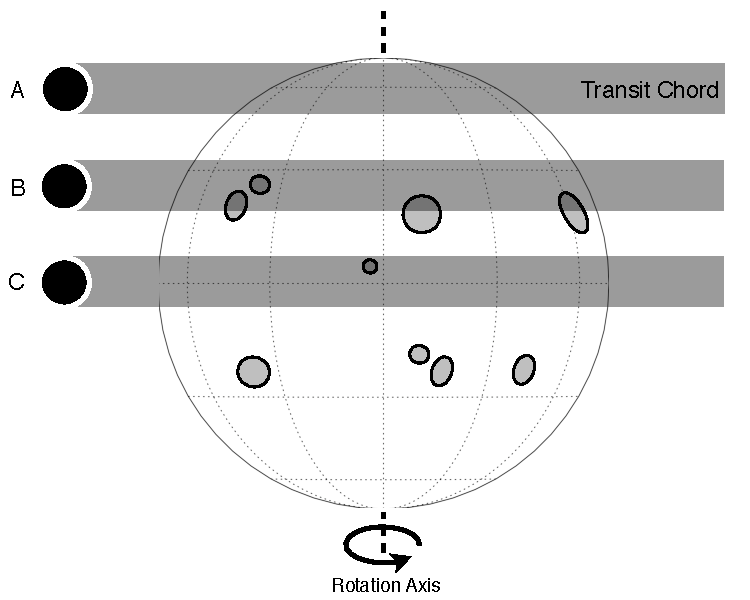
\includegraphics[width=3.5in]{diagram1}
\caption{
Schematic diagram of star with active starspot latitudes centered at $\sim$25$^\circ$ latitude, and three transiting exoplanets with impact parameters ranging between nearly b=1 (A) to  b=0 (C). The planet size is typical of a hot Jupiter, with $r_p/r_\star\approx0.11$.
}
\label{fig:diagram1}
\end{figure}


Naturally, to detect a starspot bump in transit, the transit chord projected onto the star must intersect regions on the surface containing starspots. In Figure \ref{fig:diagram1} we demonstrate three identical transiting exoplanets for a face-on star, whose transits map different ranges in latitude on the star. The spots are placed at typical latitudes for those found on the Sun, centered at $\sim$25$^\circ$ latitude. In this case, the intermediate transit (planet B) with an impact factor of $b=0.5$ intersects the northern active latitude of the star. 






%More commonly, for systems where the transits are aligned with the stellar equator (low $\lambda$, and low impact parameter, $b$), such as Kepler-17, the same spot can be detected in subsequent transits, but spots are only detectable within a narrow range of latitudes \citep{davenport_phd}, as shown in Figure \ref{fig:diagram1}. 


Now lets use LOTS of transits, but vary the impact parameter

note: a uniform distribution of impact parameters does NOT result in a uniform mapping of latitudes. hard to see high-$B$ spots.

also note: we ignoring the affect of stellar inclination here, but if could be a big problem

%%%%%
\begin{figure}[!t]
\centering
\includegraphics[width=3.5in]{diagram2}
\caption{
Schematic diagram of star with active starspot latitudes centered at $\sim$25$^\circ$ latitude, and three transiting exoplanets with impact parameters ranging between nearly b=1 (A) to  b=0 (C).
}
\label{fig:diagram2}
\end{figure}


%%%%%%%%%%%%%%%%%%%%%%
\section{Toy Model}
a simple toy model where i assume ZERO obliquity, explore:
* random impact parameters (span 0--1, but not uniformly of course)
* random stellar inclinations (within range, tend to align star+planet orbit)
* varying spot latitude band (from 60 deg to 10 deg, 10deg band?)

- plot the... "sensitivity" (recovery fraction?) as a function of the spot latitude for these random inclinations/impact parameters


%%%%%%%%%%%%%%%%%%%%%%
\section{Starspot Simulation}
we make some fake data with {\tt STSP}, at a few impact parameters, to demonstrate the kind of signal we expect in transit.


%%%%%%%%%%%%%%%%%%%%%%
\section{\Kepler Transiting Systems}
we tried it with \Kepler. It didn't work great, but we have a few thoughts as to why




%%%%%%%%%%%%%%%%%%%%%%
\section{Summary}
\label{sec:summary}


%%%%%%%%%%%%%%%%%
\acknowledgments

JRAD is supported by an NSF Astronomy and Astrophysics Postdoctoral Fellowship under award AST-1501418. 


%%%%%%%%%%%%%%%%%
\bibliography{/Users/james/Dropbox/references.bib}

\end{document}
